\documentclass[../report.tex]{subfiles}
\begin{document}	
	
\chapter{Fabrication}\label{sec:fab_process}

The \gls{mems} tunable device was fabricated using a standardized two step dry etch process on \gls{soi} for the silicon device layer (resulting in two heights) and a wet $\chem{SiO_2}$ under-etch \cite{errando-herranz_low-power_2015}. The first lithography step defines the asymmetric shape of the ridge waveguides. The second lithography step and the wet under-etch defines the slab sections and free standing cantilever. The cantilever is delimited by the fully etched slot waveguides, and its free suspended area is determined by the placement of etch holes. The details of the fabrication process steps are described in the following section.

\begin{figure}[h] %h
	\centering
	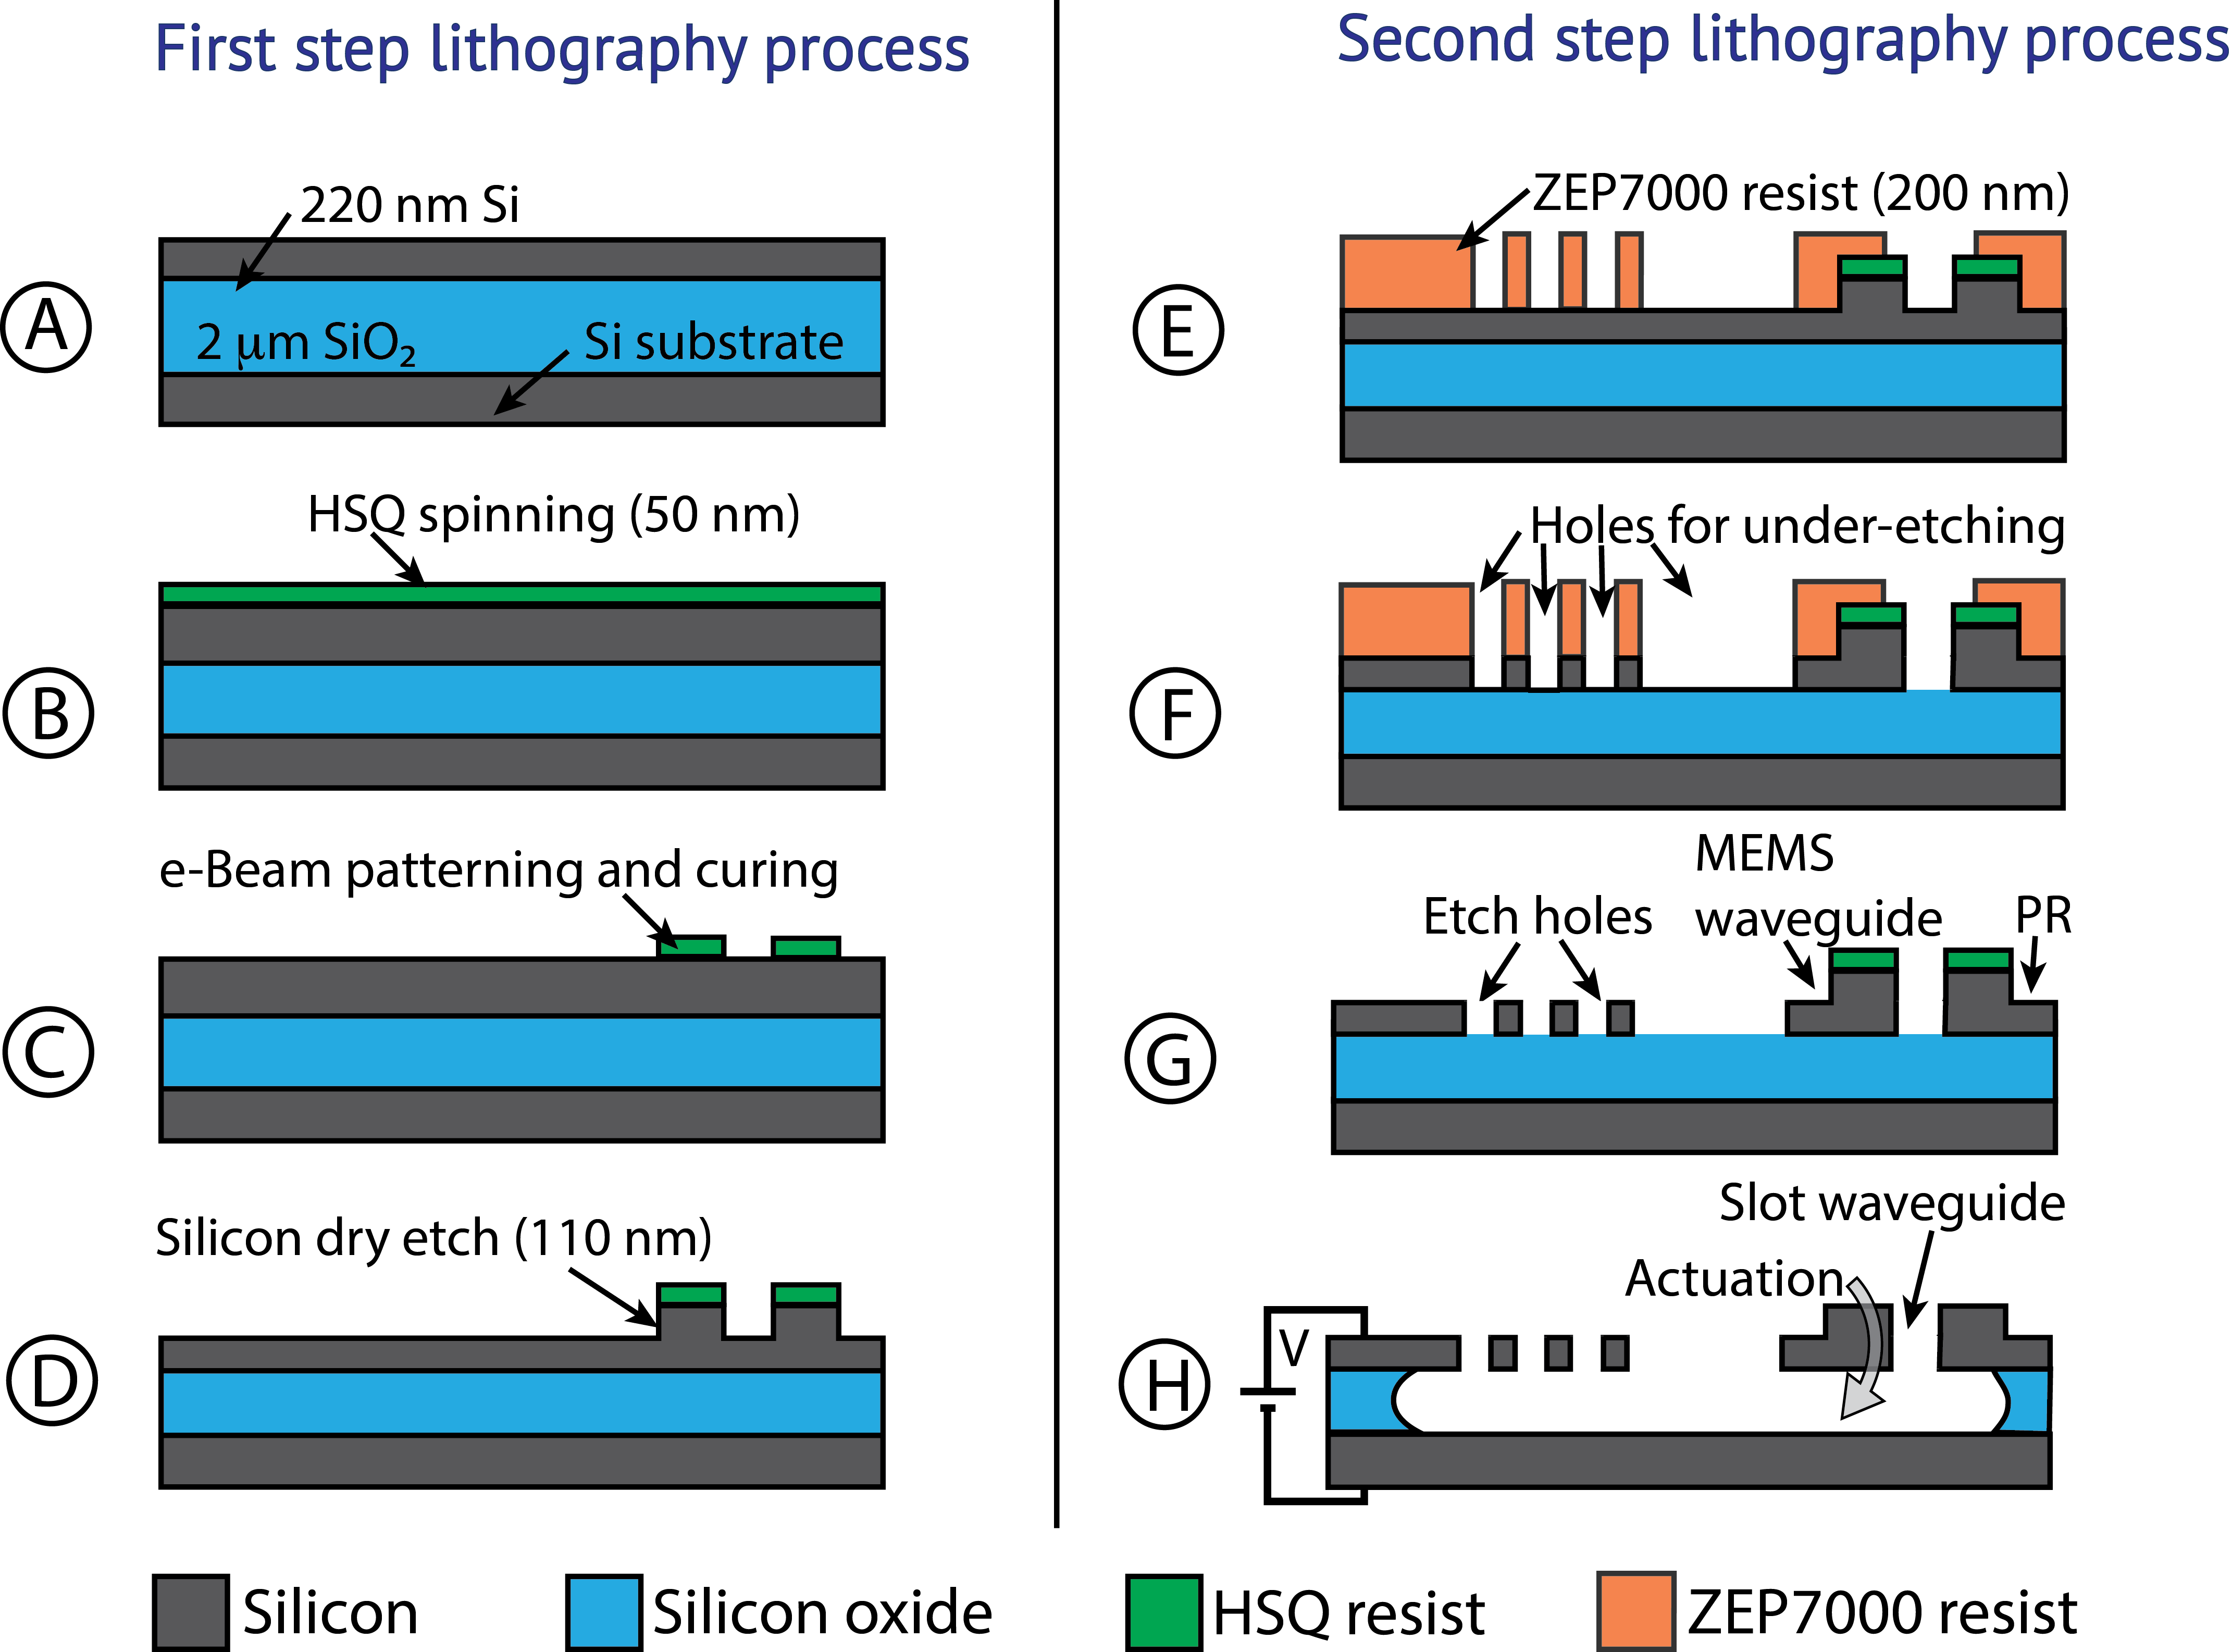
\includegraphics[width=1.0\textwidth]{5-fabrication}
	\caption{A cross-sectional schematic of the fabrication process}
	\label{fig:5_fabrication}
\end{figure}

% The fabrication process starts with a clean SOI chip with a \SI{220}{\nano \meter} crystalline silicon device layer and \SI{2}{\micro \meter} buried oxide (\ref{fig:4_fabrication} A). This is a standard substrate specification used by the Epixfab silicon photonics foundries. Electron beam patterning of a \SI{50}{\nano \meter} layer of a high-resolution negative electron beam resist (\gls{hsq}) defines the waveguide structures (\ref{fig:4_fabrication} B). The pattern is then transferred to the device layer by timed dry etch of silicon, resulting in ridge waveguide structures with \SI{110}{\nano \meter} height on a \SI{110}{\nano \meter} thick silicon slab ((\ref{fig:4_fabrication} C)). The patterned \gls{hsq} remains on the chip for the next lithography step.
%$\chem{H_2} + (1/2)\,\chem{O_2} = \chem{H_2O}$

\section{Piranha bath}			
The fabrication process starts with cleaning the \gls{soi} chip which has \SI{220}{\nano \meter} crystalline silicon device layer and \SI{2}{\micro \meter} buried oxide, in the piranha solution (Fig. \ref{fig:5_fabrication} A). Piranha solution is a mixture of sulfuric acid ($\chem{H_2SO_4}$) and hydrogen peroxide ($\chem{H_2O_2}$), used to clean organic residues off substrates. Because the mixture is a strong oxidizing agent, it will remove most organic matter, and it will also hydroxylate most surfaces (add OH groups), making them highly hydrophilic (water-loving) \cite{piranha_bath}. 
 
\section{HSQ resist spin}
A \gls{hsq} negative resist is spun on the \gls{soi} chip to create a thickness of \SI{50}{\nano \meter}. This is achieved by spinning the chip on a spinner at 4000rpm for 30 seconds. The \gls{hsq} layer is hardened by baking the chip on a hot plate at $\chem{170^{\circ}}$ C for 5 minutes. To measure the thickness of resist a scratch is made on the chip and checked for depth variations using mechanical profilometer (KLA-Tencor). This is done to verify the profile depth of the resist mask.

\section{First e-beam exposure}
To pattern the chip, selective portions of the chip are exposed using e-beam lithography. The patterns are drawn using a CAD software (Raith 150 e-beam lithography). E-beam exposure exceeds patterning capability of optical lithography and creates patterns in sub-microns scale. Initially, one corner of the chip is scratched to align the chip and find particles on the chip to focus the beam correctly. Write-field alignment is a very central adjustment in the process of getting the best possible e-beam lithographic result. It is the adjustment of the electromagnetic/electrostatic deflections system inside the column to the high precision X-Y-Z stage. The stage is considered to be ``correct'' and the e-beam deflection system is aligned to it. To increase the dose in certain portions of the chip, the scanning speed is slowed down so that more electrons can strike the \gls{hsq} surface and expose it with a higher dose. The chip is developed using ma-D 525 (micro-resist) which dissolves non-hardened \gls{hsq}. The chip is then put in water to wash ma-D 525 and dried using nitrogen. Finally, the exposed \gls{hsq} on the chip is hardened more by putting it in an oven for 40 minutes at $\chem{400^{\circ}}$ C. Inside the oven the chip is covered with ceramic glass to avoid deposition of dust cloud. After this step the chip resembles the diagram in Fig. \ref{fig:5_fabrication} C. Again a mechanical profilometer is used to verify the thickness of \gls{hsq}.    

\section{First dry etch step}
The device pattern is finally transferred to the device layer by a timed ($\chem{HBr}$) dry etching of silicon ($\approx$ 35 seconds), resulting in ridge waveguides with \SI{110}{\nano \meter} height on a \SI{110}{\nano \meter} thick silicon slab (Fig. \ref{fig:5_fabrication} D). The patterned \gls{hsq} remains on the chip for the next lithography step. Finally, optical profiling is performed to find out the depth of the silicon etch. This process marks the end of the first step lithography process.

\section{ZEP7000 spin}
A ZEP7000 resist (positive) is applied on the chip by using an Eppendorf pipette. To achieve a ZEP profile of \SI{200}{\nano \meter} thickness the spinner is set at 3000 rpm for 45 seconds. The sample is baked at $\chem{170^{\circ}}$ C for 3 minutes to make the ZEP layer harder. After this, a scratch is then made on the sample and the profile depth is measured using a mechanical profilometer.

\section{Second e-beam exposure}
Initially, before the second e-beam exposure the beam is focused correctly and alignment to existing structures is performed because it is a two-step fabrication process. Some unique and easily recognizable feature like plus symbol is selected as a mark, patterned in the first exposure. Write-field alignment is performed in all the cells manually for maximum dimensional precision \cite{write_field}. Since ZEP is a positive resist, the exposed portions are developed using p-Xylene solvent and MIBK. After developing the chip, the cross-section looks like Fig. \ref{fig:5_fabrication} E.

\section{Second dry etch step}
The double step device pattern is obtained in the device layer when the unmasked silicon (without ZEP resist) is etched. This is done via another dry etch step similar to the previous one ($\approx$ 35 seconds). The goal of this dry etch process is to etch through the remaining silicon via the holes created using ZEP resist. The ZEP polymer is cleaned via resist stripping using oxygen plasma. After this process the device cross-section looks like Fig. \ref{fig:5_fabrication} F. 

\section{Wet etching and critical point drying}
The final step in the fabrication is the of removal of the \gls{hsq} and the underlying $\chem{SiO_2}$ to form the free-standing \gls{mems} waveguide with cantilever and the \gls{pr} waveguide with a gap of \SI{100}{\nano \meter}. The process starts with wet etching of \gls{hsq} and $\chem{SiO_2}$ using HF for 200 seconds. The HF is diluted using cold water and then the chip is transferred to isopropanol ($\chem{CH_3CHOHCH_3}$). The surface tension of the isopropanol in a micro device is at the point at which a change from liquid to gaseous state can destroy the device through capillary forces. Also, drying free standing waveguides in air or under vacuum can drastically alter their structures or even destroy them completely. A gentle method for such purposes is critical point drying. By increasing the pressure and temperature of the substrate it is possible to dry without crossing a phase boundary. This is possible because once the critical point has been passed, the density of liquid and gas are the same. $\chem{CO_2}$ is a good transitional fluid for which the critical point temperature and pressure are relatively low and hence the \gls{mems} structures are not destroyed. Hence, in the critical point drying machine, initially the isopropanol is replaced with liquid $\chem{CO_2}$ slowly and then liquid $\chem{CO_2}$ is dried. After the critical point drying the device is developed with the structure as in Fig. \ref{fig:5_fabrication} H. 

\section{Final product}

To view the patterns in the device after fabrication \gls{sem} images are developed by scanning the sample with a focused beam of electrons. This helps in analyzing the results conducted during the experiment. It can be seen in Fig. \ref{fig:5_te_pr_pbs} that \gls{te} tapers are not suspended. The cross-sectional pattern of the \gls{mems} \gls{tpr} is viewable in Fig. \ref{fig:5_te_pr_zoom}. However, the \gls{tm} gratings and tapers both are suspended and can be viewed in Fig. \ref{fig:5_tm_pr_pbs} and Fig. \ref{fig:5_tm_gratings_suspended}. In Fig. \ref{fig:5_tm_pr_pbs} the bridges are visible which holds the suspending waveguide and taper. In Fig. \ref{fig:5_tm_gratings_suspended}, the \gls{tm} gratings can be seen. The gratings are suspended because of under-etching through the holes. The cross-section of the waveguide at the cantilever section can be seen in Fig. \ref{fig:5_tm_pr_zoom}. A suspended \gls{pbs} can be viewed in Fig. \ref{fig:5-pbs-suspended}.

\begin{figure}[H] %h
	\centering
	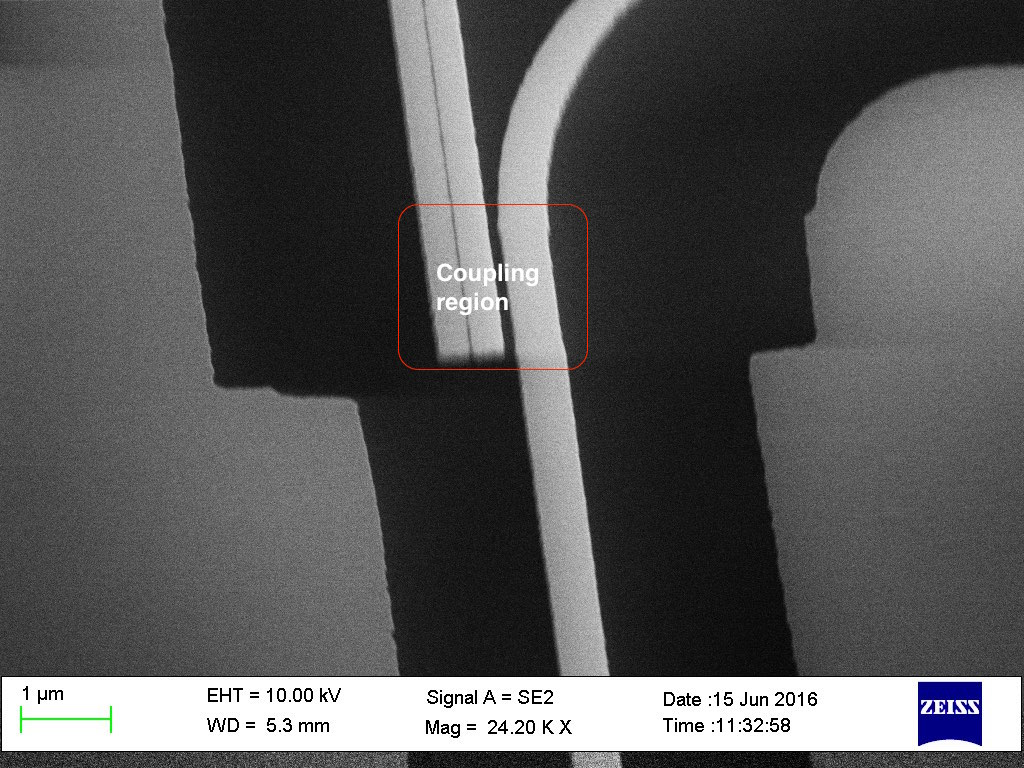
\includegraphics[width=0.65\textwidth]{5-pbs-suspended}
	\caption{Suspended \gls{pbs} with \gls{tm} cross-port and \gls{te} through}
	\label{fig:5-pbs-suspended}
\end{figure}

\begin{figure}[H] %h
	\centering
	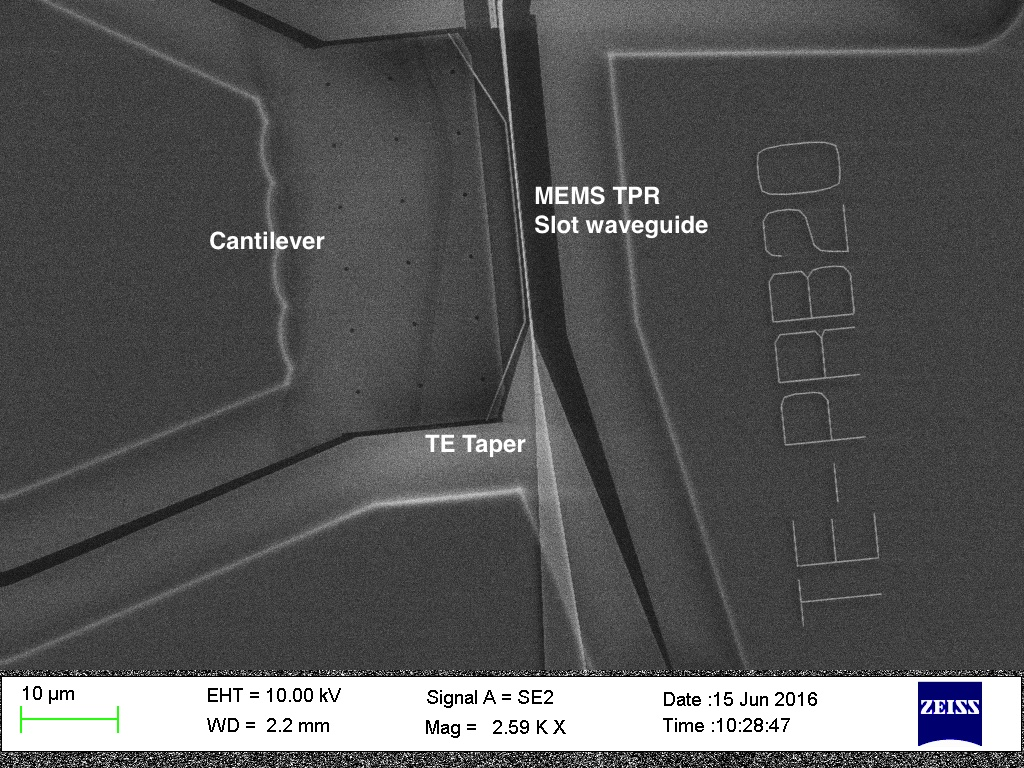
\includegraphics[width=0.8\textwidth]{5-te-pr-pbs}
	\caption{\gls{te} input with tapers, \gls{pbs} and \gls{mems} cantilever viewed in \gls{sem}}
	\label{fig:5_te_pr_pbs}
\end{figure}

\begin{figure}[H] %h
	\centering
	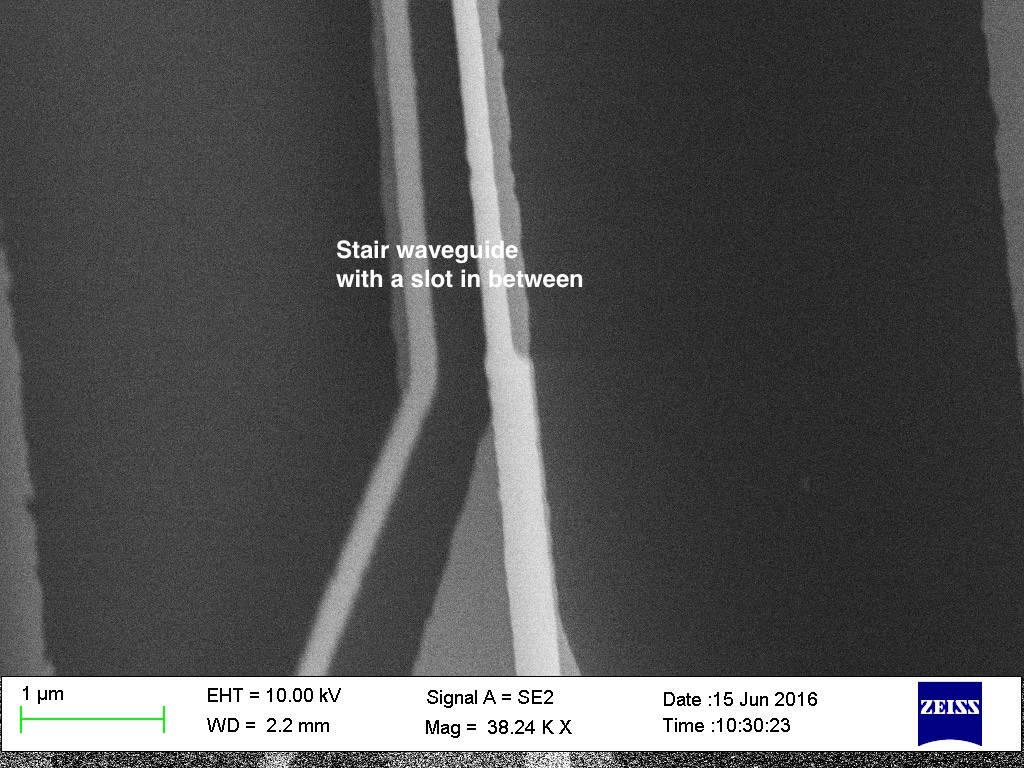
\includegraphics[width=0.8\textwidth]{5-te-pr-zoom}
	\caption{Cross-section in the slot region with \gls{mems} tuned waveguide and core waveguide for \gls{te} input}
	\label{fig:5_te_pr_zoom}
\end{figure}

\begin{figure}[H] %h
	\centering
	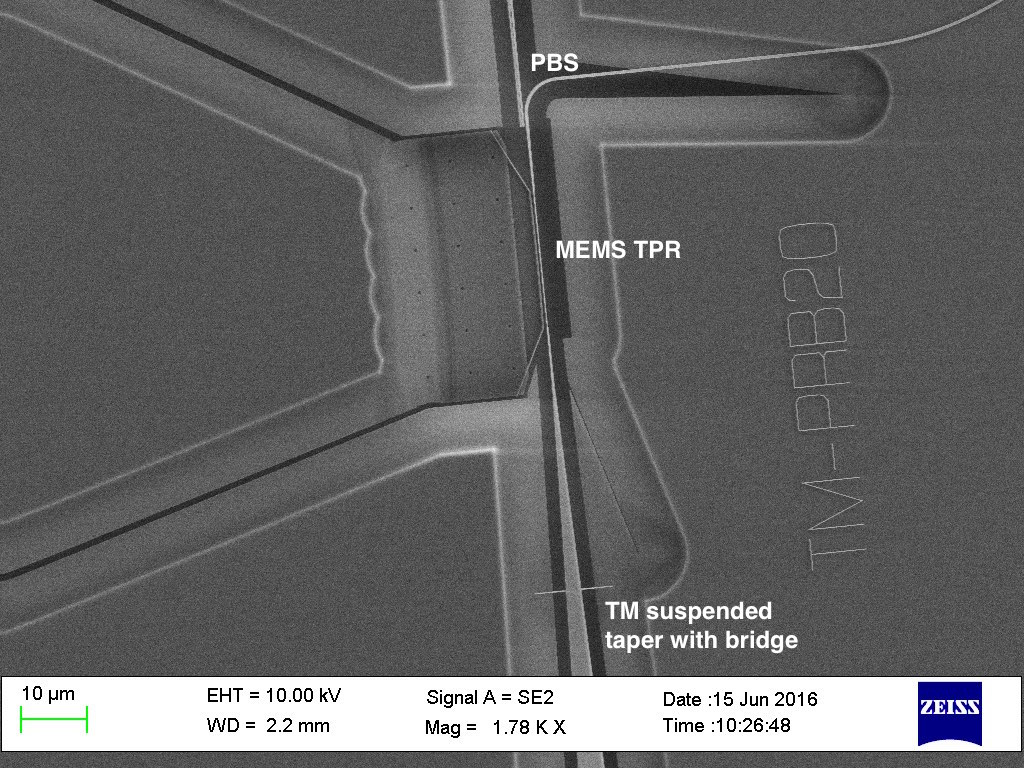
\includegraphics[width=0.8\textwidth]{5-tm-pr-pbs}
	\caption{\gls{tm} input with tapers, \gls{pbs} and \gls{mems} cantilever viewed under \gls{sem}}
	\label{fig:5_tm_pr_pbs}
\end{figure}

\begin{figure}[H] %h
	\centering
	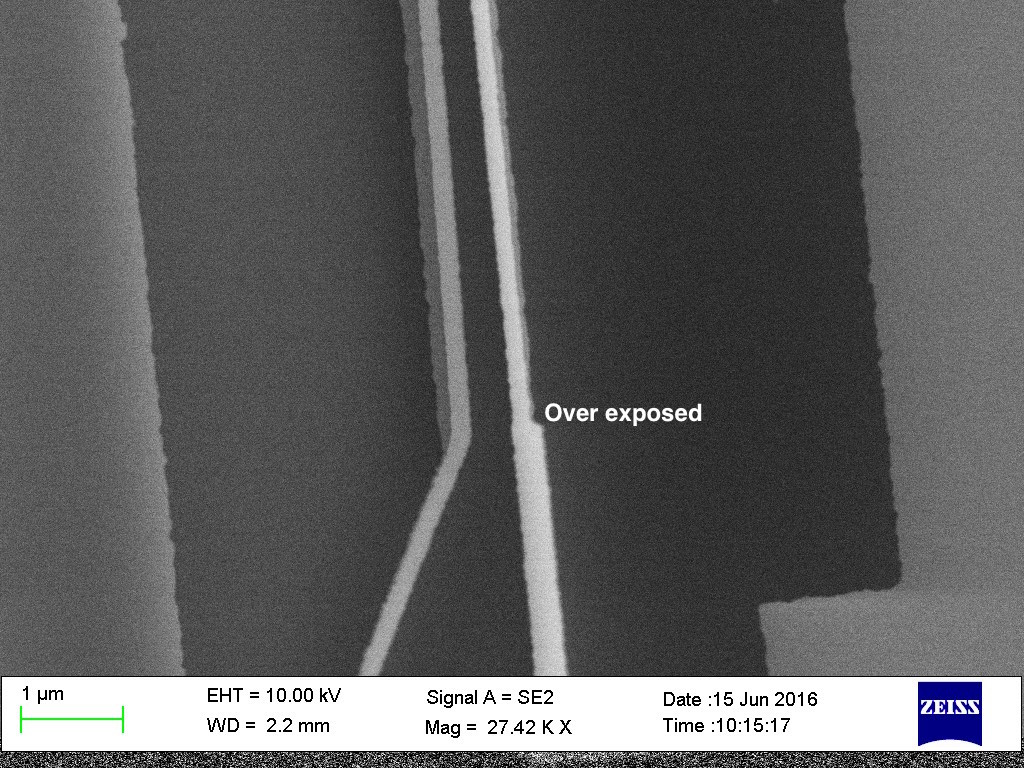
\includegraphics[width=0.8\textwidth]{5-tm-pr-zoom}
	\caption{Cross-section in the slot region with \gls{mems} tuned waveguide and core waveguide for \gls{tm} input}
	\label{fig:5_tm_pr_zoom}
\end{figure}

\begin{figure}[h] %h
	\centering
	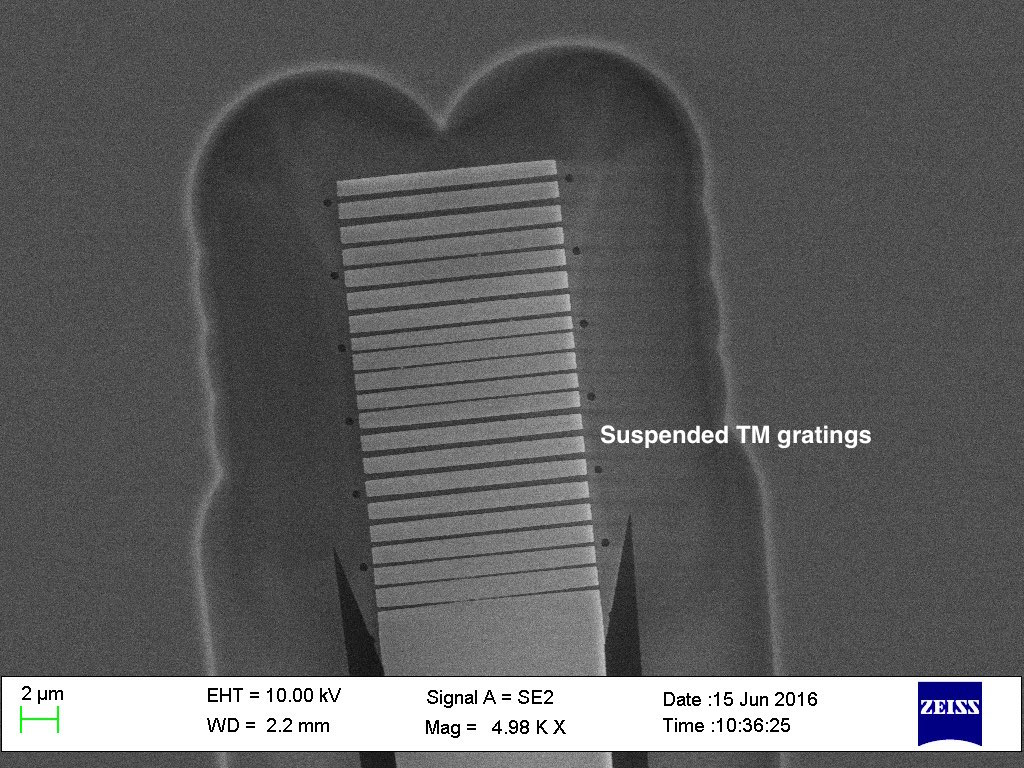
\includegraphics[width=0.8\textwidth]{5-tm-gratings-suspended}
	\caption{\gls{tm} suspended gratings viewed under \gls{sem}}
	\label{fig:5_tm_gratings_suspended}
\end{figure}

\begin{figure}[h] %h
	\centering
	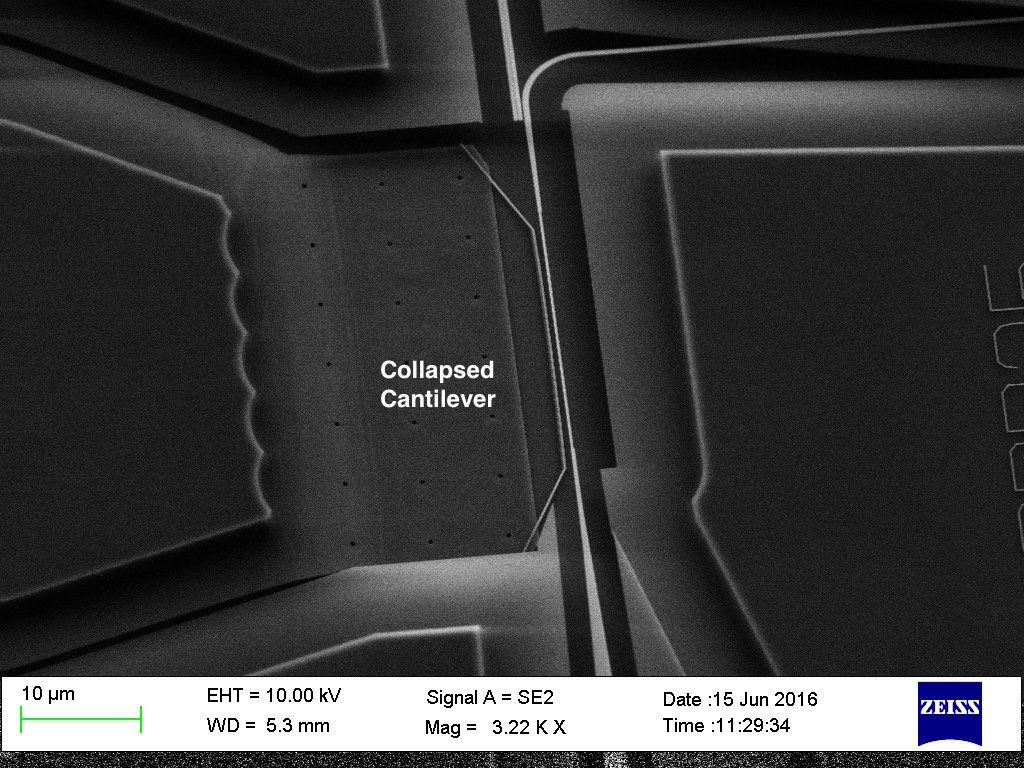
\includegraphics[width=0.8\textwidth]{5-tm-sticked-mems}
	\caption{Stiction problem on applying a voltage more than the pull in voltage}
	\label{fig:5_tm_sticked_mems}
\end{figure}

\end{document}
